% Author: Grayson Orr
% Course: ID511001: Programming 2

\documentclass{article}
\author{}

\usepackage{graphicx}
\usepackage{wrapfig}
\usepackage{enumerate}
\usepackage{hyperref}
\usepackage[margin = 2.25cm]{geometry}
\usepackage[table]{xcolor}
\usepackage{soul}
\usepackage{fancyhdr}
\usepackage{fancyvrb}
\hypersetup{
  colorlinks = true,
  urlcolor = blue
}
\setlength\parindent{0pt}
\pagestyle{fancy}
\fancyhf{}
\rhead{College of Engineering, Construction \& Living Sciences\\Bachelor of Information Technology}
\lfoot{Project 1 (C\# Console App): Learner Gradebook\\Version 1, Semester One, 2023}
\rfoot{\thepage}
 
\begin{document}

\begin{figure}
    \centering
    
\includegraphics[width=50mm]{../../resources/img/logo.png}
\end{figure}

\title{College of Engineering, Construction \& Living Sciences\\Bachelor of Information Technology\\ID511001: Programming 2\\Level 5, Credits 15\\\textbf{Project 1 (C\# Console App): Learner Gradebook}}
\date{}
\maketitle

\section*{Assessment Overview}
In this assessment, you will design \& develop a learner gradebook \textbf{Console App} using \textbf{C\#}. 

\section*{Learning Outcomes}
At the successful completion of this course, learners will be able to:
\begin{enumerate}
    \item Build interactive, event-driven GUI applications using pre-built components.
    \item Declare \& implement user-defined classes using encapsulation, inheritance \& polymorphism.
\end{enumerate}

\section*{Assessments}
\renewcommand{\arraystretch}{1.5}
\begin{tabular}{|c|c|c|c|}
	\hline
	\textbf{Assessment}                                 & \textbf{Weighting} & \textbf{Due Date}            & \textbf{Learning Outcomes} \\ \hline
	\small Project 1 (C\# Console App): Learner Gradebook  & \small 25\%        & \small 26-04-2023 (Wednesday at 4.59 PM)   & \small 1 \& 2                   \\ \hline
	\small Project 2 (C\# Windows Forms App): Pong & \small 35\%        & \small 14-06-2023 (Wednesday at 4.59 PM)   & \small 1 \& 2                   \\ \hline
	\small Theory Examination                        & \small 30\%        & \small 21-06-2023 (Wednesday at 4.45 PM)  & \small 1 \& 2                   \\ \hline
	\small Classroom Tasks                       & \small 10\%        & \small 07-06-2023 (Wednesday at 4.59 PM)  & \small 1 \& 2                   \\ \hline
\end{tabular} 

\section*{Conditions of Assessment}
You will complete this assessment during your learner-managed time. However, there will be time during class to discuss the requirements \& your progress on this assessment. This assessment will need to be completed by \textbf{Wednesday, 26 April 2022} at \textbf{4.59 PM}.

\section*{Pass Criteria}
This assessment is criterion-referenced (CRA) with a cumulative pass mark of \textbf{50\%} over all assessments in \textbf{ID511001: Programming 2}.

\section*{Authenticity}
All parts of your submitted assessment \textbf{must} be completely your work. If you use code snippets from \textbf{GitHub}, \textbf{StackOverflow} or other online resources, you \textbf{must} reference it appropriately using \textbf{APA 7th edition}. Provide your references in the \textbf{README.md} file in your repository. Failure to do this will result in a mark of \textbf{zero} for this assessment.

\section*{Policy on Submissions, Extensions, Resubmissions \& Resits}
The school's process concerning submissions, extensions, resubmissions \& resits complies with \textbf{Te Pūkenga} policies. Learners can view policies on the \textbf{Te Pūkenga} website located at \href{https://www.op.ac.nz/about-us/governance-and-management/policies}{https://www.op.ac.nz/about-us/governance-and-management/policies}.

\section*{Submission}
You \textbf{must} submit all app files via \textbf{GitHub Classroom}. Here is the URL to the repository you will use for your submission – \href{https://classroom.github.com/a/eFe1Oh97}{https://classroom.github.com/a/eFe1Oh97}.  Create a \textbf{.gitignore} \& add the ignored files in this resource - \href{https://raw.githubusercontent.com/github/gitignore/main/VisualStudio.gitignore}{https://raw.githubusercontent.com/github/gitignore/main/VisualStudio.gitignore}. The latest app files in the \textbf{master} or \textbf{main} branch will be used to mark against the \textbf{Functionality} criterion. Please test before you submit. Partial marks \textbf{will not} be given for incomplete functionality. Late submissions will incur a \textbf{10\% penalty per day}, rolling over at \textbf{5:00 PM}.

\section*{Extensions}
Familiarise yourself with the assessment due date. Contact the course lecturer before the due date if you need an extension. If you require more than a week's extension, you will need to provide a medical certificate or support letter from your manager.

\section*{Resubmissions}
Learners may be requested to resubmit an assessment following a rework of part/s of the original assessment. Resubmissions are to be completed within a negotiable short time frame \& usually \textbf{must} be completed within the timing of the course to which the assessment relates. Resubmissions will be available to learners who have made a genuine attempt at the first assessment opportunity \& achieved a \textbf{D grade (40-49\%)}. The maximum grade awarded for resubmission will be \textbf{C-}.

\section*{Resits}
Resits \& reassessments \textbf{are not} applicable in \textbf{ID511001: Programming 2}.

\section*{Instructions}
You will need to submit an app \& documentation that meet the following requirements:\\

\subsection*{Functionality - Learning Outcomes 1 \& 2 (40\%)}
\begin{itemize}
    \item The app \textbf{must} open without code or file structure modification in \textbf{Visual Studio}.
    \item Create the following classes:
    \begin{itemize}
        \item \textbf{AssessmentMarks} which has the following field:
        \begin{itemize}
            \item \textbf{assessmentMarks} of type \textbf{List$<$int$>$}
        \end{itemize}
        \item \textbf{Person} which is an \textbf{abstract} class \& has the following fields \& method:
        \begin{itemize}
            \item \textbf{id} of type \textbf{int}
            \item \textbf{firstName} of type \textbf{string}
            \item \textbf{lastName} of type \textbf{string}
            \item \textbf{DisplayDetails()} which is a \textbf{public abstract} method, has no arguments \& returns a \textbf{string}
        \end{itemize}    
        \item \textbf{Learner} which inherits from \textbf{Person} \& has the following additional fields \& method:
        \begin{itemize}
            \item \textbf{prog1AssessmentMarks} of type \textbf{AssessmentMarks}
            \item \textbf{prog2AssessmentMarks} of type \textbf{AssessmentMarks}
            \item \textbf{DisplayDetails()} which is an \textbf{override} method, has no arguments \& returns a \textbf{Learner's} \textbf{id}, \textbf{first name} \& \textbf{last name}
        \end{itemize}
        \item \textbf{Lecturer} which inherits from \textbf{Person} \& has the following additional fields \& method:
        \begin{itemize}
            \item \textbf{position} of type \textbf{string}
            \item \textbf{salary} of type \textbf{int}
            \item \textbf{DisplayDetails()} which is an \textbf{override} method, has no arguments \& returns a \textbf{Lecturer's} \textbf{id}, \textbf{first name}, \textbf{last name}, \textbf{position} \& \textbf{salary}
        \end{itemize}
    \end{itemize}
    \item Read a text file called \textbf{learners.txt} which contains information about five learners. This information includes \textbf{id}, \textbf{first name}, \textbf{last name}, three \textbf{ID510001: Programming 1 assessment marks} \& three \textbf{ID511001: Programming 2 assessment marks}. \textbf{Note:} \textbf{learners.txt} \textbf{must} be located in the \textbf{bin/Debug} folder.
    \item Create a \textbf{List} of \textbf{Learner} objects \& populate it with the information from the \textbf{learners.txt} file.
    \item Read a text file called \textbf{lecturers.txt} which contains information about three lecturers. This information includes \textbf{id}, \textbf{first name}, \textbf{last name}, \textbf{position} \& \textbf{salary}. \textbf{Note:} \textbf{lecturers.txt} \textbf{must} be located in the \textbf{bin/Debug} folder.
    \item Create a \textbf{List} of \textbf{Lecturer} objects \& populate it with the information from the \textbf{lecturers.txt} file.
    \item An \textbf{AssessmentMarks} object has several behaviours such as getting all marks, all grades, highest mark(s), lowest mark(s), fail mark(s), average marks \& average grades. Create the following \textbf{public} methods in the \textbf{AssessmentMarks} class:
    \begin{itemize}
        \item \textbf{GetAllMarks()} which has no arguments \& returns a \textbf{List$<$int$>$} 
        \item \textbf{GetAllGrades()} which has no arguments \& returns a \textbf{List$<$string$>$}
        \item \textbf{GetHighestMarks()} which has no arguments \& returns a \textbf{List$<$int$>$}
        \item \textbf{GetLowestMarks()} which has no arguments \& returns a \textbf{List$<$int$>$}
        \item \textbf{GetFailMarks()} which has no arguments \& returns a \textbf{List$<$int$>$}
        \item \textbf{GetAverageMark()} which has no arguments \& returns a \textbf{double}
        \item \textbf{GetAverageGrade()} which has no arguments \& returns a \textbf{string}
    \end{itemize}
    \item A grade is calculated using the following grade table:\\\\
    \renewcommand{\arraystretch}{1.5}
    \begin{tabular}{|c|c|}
        \hline
        \textbf{Grade} & \textbf{Mark Range} \\ \hline
        A+ & 90-100  \\ \hline
        A & 85-89  \\ \hline
        A- & 80-84 \\ \hline
        B+ & 75-79   \\ \hline
        B & 70-74  \\ \hline
        B- & 65-69  \\ \hline
        C+ & 60-64  \\ \hline
        C & 55-59 \\ \hline
        C- & 50-54  \\ \hline
        D & 40-49   \\ \hline
        E & 0-39   \\ \hline
    \end{tabular}
    \\\\ \textbf{Note:} The \textbf{lowest passing mark} is 50. If a learner achieves a mark of 50 in each assessment, i.e., 50, 50, 50 for a course, i.e., \textbf{ID510001: Programming 1} the \textbf{lowest passing mark} is 50 and the \textbf{highest passing mark} is 50.  
    \item The app \textbf{must} display the following menu options:
    \begin{itemize}
        \item 1. Display all marks
        \item 2. Display all grades
        \item 3. Display highest, lowest and fail marks
        \item 4. Display average marks
        \item 5. Display average grades
        \item 6. Add a learner
        \item 7. Remove a learner
        \item 8. Display lecturer details
        \item 0. Exit
    \end{itemize}
    \textbf{Note:} In the \textbf{Program.cs} file, you will need to create methods to achieve this functionality. Also, the app \textbf{must} be able to handle invalid user input. If the user enters an invalid option, a message \textbf{must} be displayed.
    \begin{figure}[ht]
        \centering
        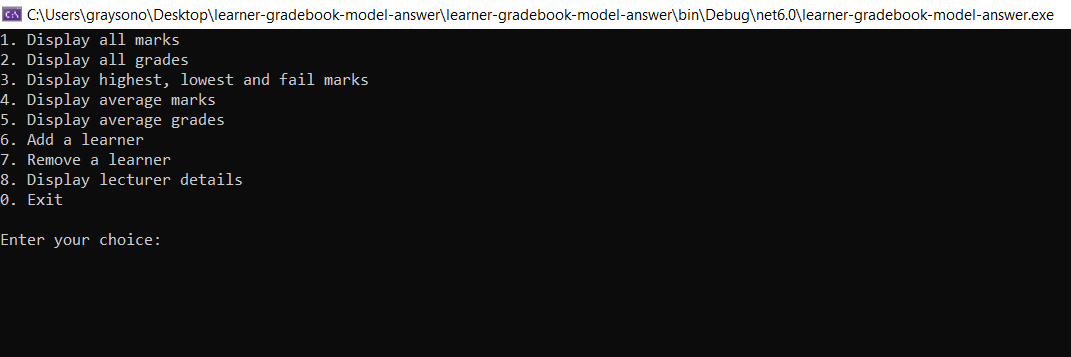
\includegraphics[width=150mm,height=50mm]{../../resources/img/project-1/1.PNG}
    \end{figure} 
    \item When the user selects \textbf{1. Display all marks}, the app \textbf{must} display all marks for all learners. The marks \textbf{must} be displayed as follows:
    \begin{figure}[ht]
        \centering
        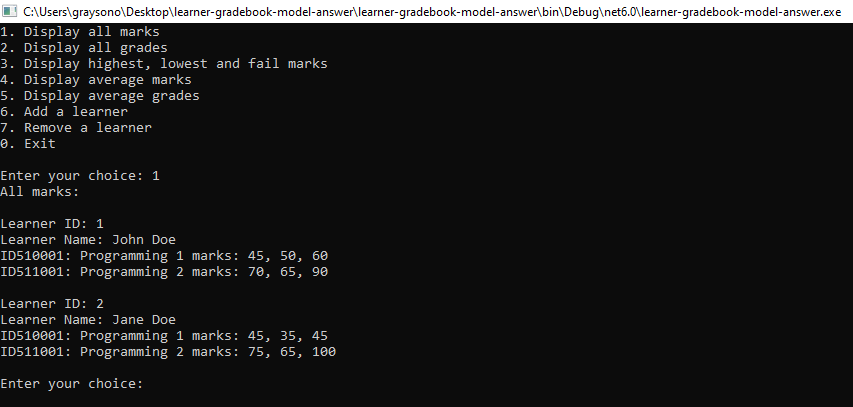
\includegraphics[width=150mm,height=75mm]{../../resources/img/project-1/2.PNG}
    \end{figure}
    \newpage
    \item When the user selects \textbf{2. Display all grades}, the app \textbf{must} display all grades for all learners. The grades \textbf{must} be displayed as follows:
    \begin{figure}[ht] 
        \centering
        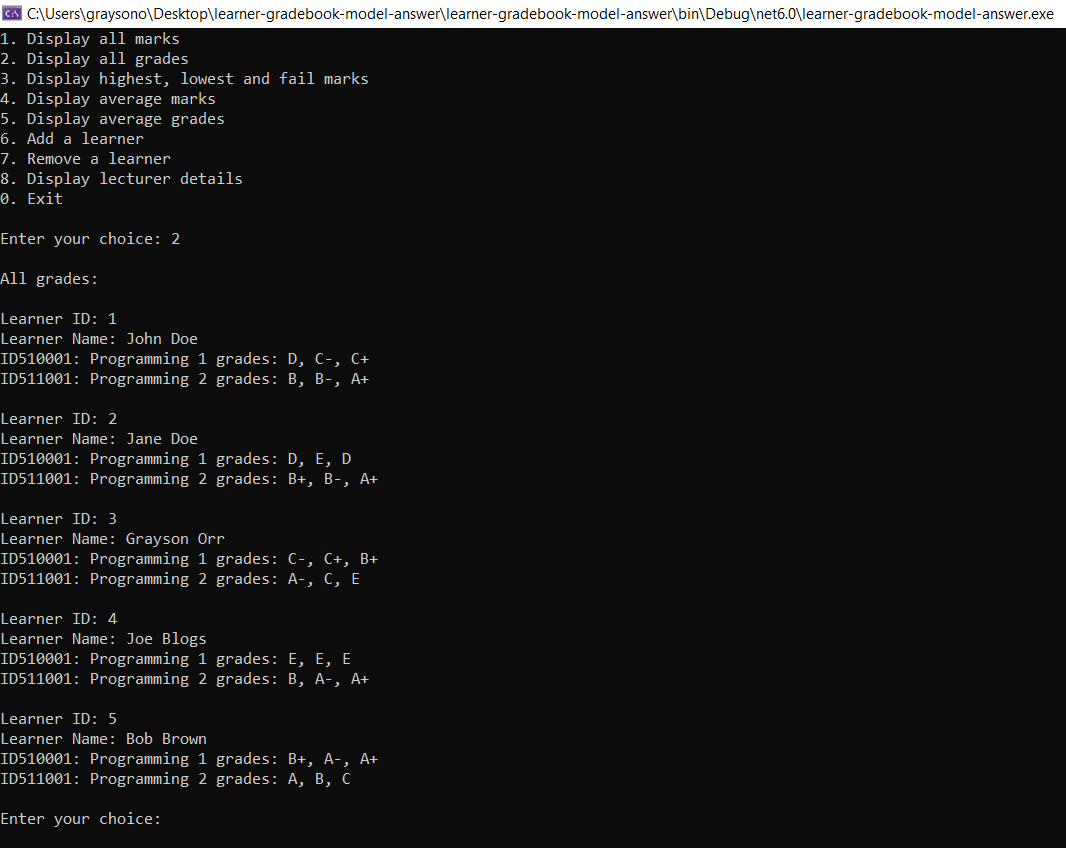
\includegraphics[width=150mm,height=75mm]{../../resources/img/project-1/3.PNG}
    \end{figure}
    \item When the user selects \textbf{3. Display highest, lowest and fail marks}, the app \textbf{must} display the highest, lowest \& fail marks for all learners. The marks \textbf{must} be displayed as follows:
    \begin{figure}[ht]
        \centering
        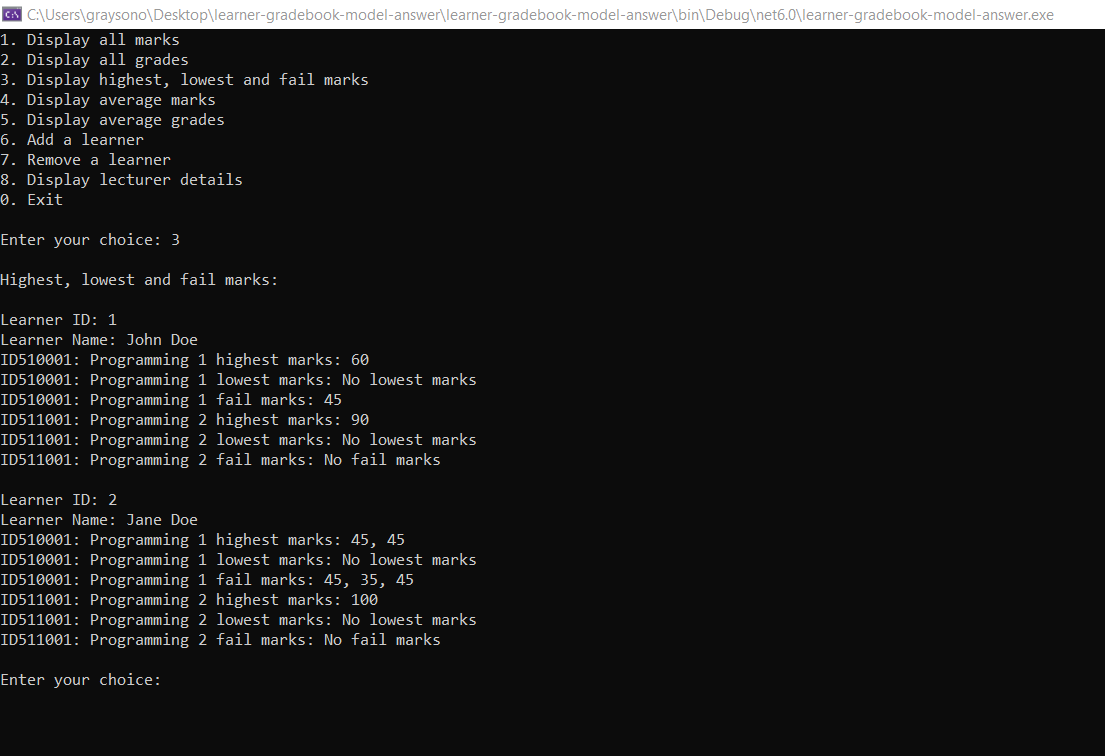
\includegraphics[width=150mm,height=90mm]{../../resources/img/project-1/4.PNG}
    \end{figure}
    \newpage
    \textbf{Note:} If there is no fail mark(s), the \textbf{Fail marks:} \textbf{must} be displayed as \textbf{No fail marks}. If there is no lowest mark(s), the \textbf{Lowest marks:} \textbf{must} be displayed as \textbf{No lowest marks}. If there is no highest mark(s), the \textbf{Highest marks:} \textbf{must} be displayed as \textbf{No highest marks}.
    \item When the user selects \textbf{4. Display average marks}, the app \textbf{must} display the average marks for all learners. The marks \textbf{must} be displayed as follows:
    \begin{figure}[ht]
        \centering
        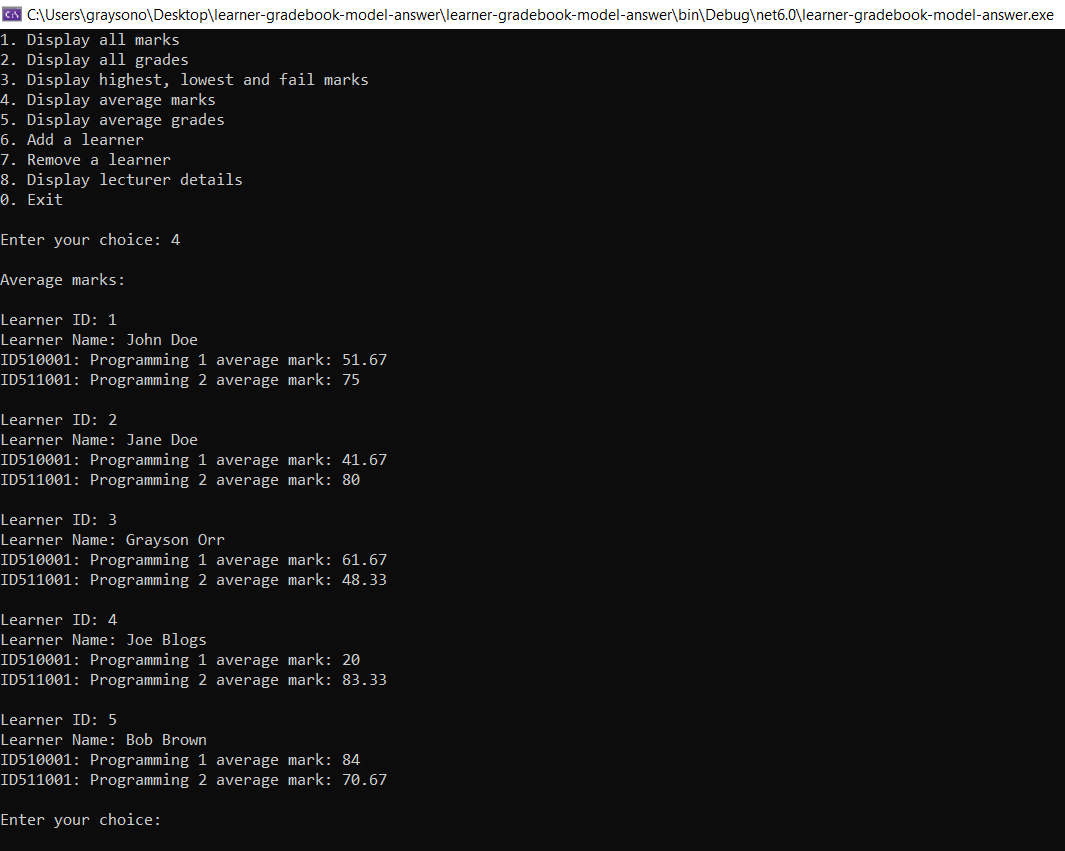
\includegraphics[width=150mm,height=75mm]{../../resources/img/project-1/5.PNG}
    \end{figure}
    \item When the user selects \textbf{5. Display average grades}, the app \textbf{must} display the average grades for all learners. The grades \textbf{must} be displayed as follows:
    \begin{figure}[ht]
        \centering
        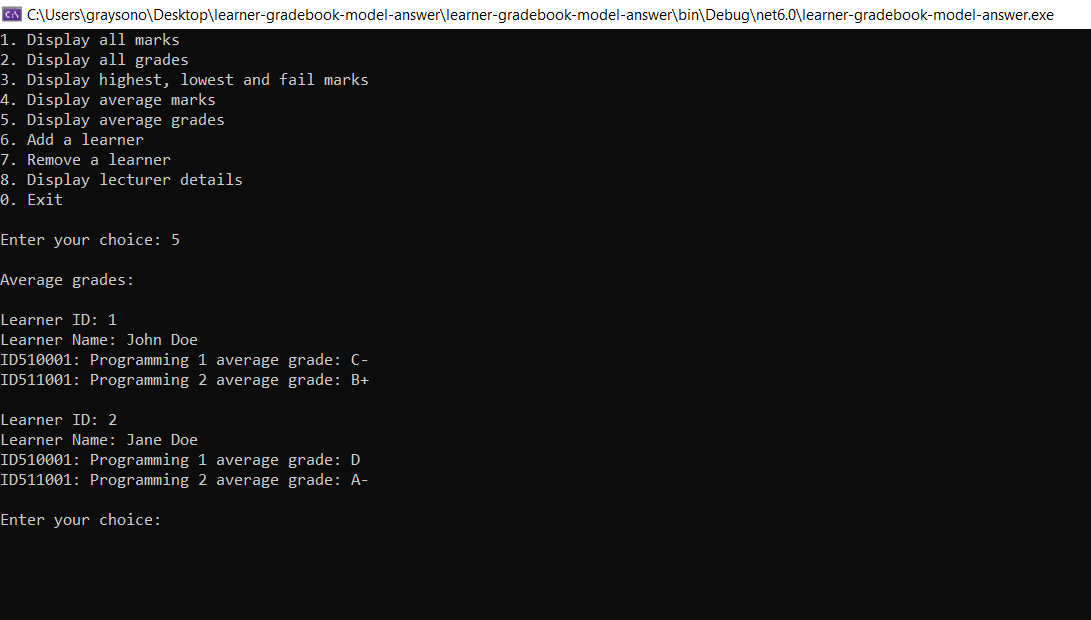
\includegraphics[width=150mm,height=75mm]{../../resources/img/project-1/6.PNG}
    \end{figure}
    \newpage
    \item When the user selects \textbf{6. Add a learner}, the app \textbf{must} prompt the user to enter the following information:
    \begin{itemize}
        \item \textbf{First name}
        \item \textbf{Last name}
        \item \textbf{ID510001: Programming 1 assessment mark 1}
        \item \textbf{ID510001: Programming 1 assessment mark 2}
        \item \textbf{ID510001: Programming 1 assessment mark 3}
        \item \textbf{ID511001: Programming 2 assessment mark 1}
        \item \textbf{ID511001: Programming 2 assessment mark 2}
        \item \textbf{ID511001: Programming 2 assessment mark 3}
    \end{itemize}
    \textbf{Note:} A \textbf{first name} \& \textbf{last name} \textbf{must} not contain numbers or special characters. An \textbf{assessment mark} \textbf{must} be between \textbf{0} \& \textbf{100}. If an \textbf{assessment mark} is invalid, an error message \textbf{must} be displayed. The learner's \textbf{id} \textbf{must} be generated automatically. However, the \textbf{id} \textbf{must} be unique. Append the learner's information to the \textbf{learners.txt} file.  
    \begin{figure}[h]
        \centering
        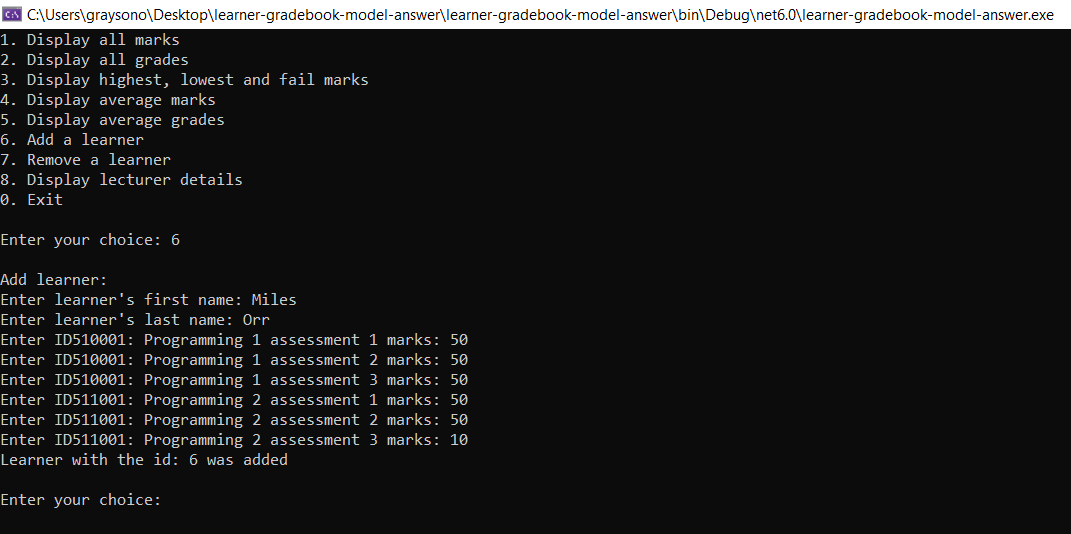
\includegraphics[width=150mm,height=110mm]{../../resources/img/project-1/7.PNG}
    \end{figure}
    \newpage
    \item When the user selects \textbf{7. Remove a learner}, the app \textbf{must} prompt the user to enter the \textbf{id} of the learner to be removed. If the learner is found, the learner \textbf{must} be removed from the \textbf{List} of \textbf{Learner} objects. If the learner is not found, an error message \textbf{must} be displayed.
    \begin{figure}[h]
        \centering
        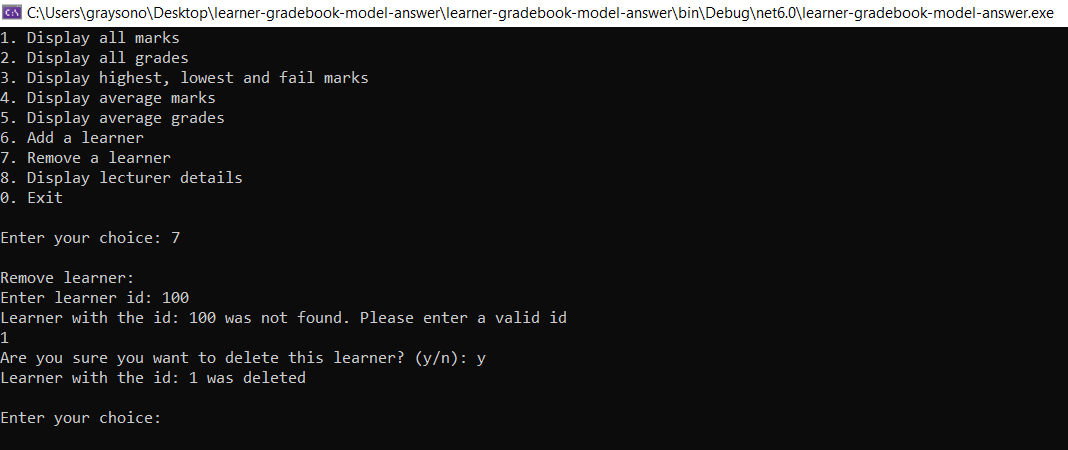
\includegraphics[width=150mm,height=85mm]{../../resources/img/project-1/8.PNG}
    \end{figure}
    \newpage
    \item When the user selects \textbf{8. Display lecturer details}, the app \textbf{must} display the lecturer's details. The details \textbf{must} be displayed as follows:
    \begin{figure}[h]
        \centering
        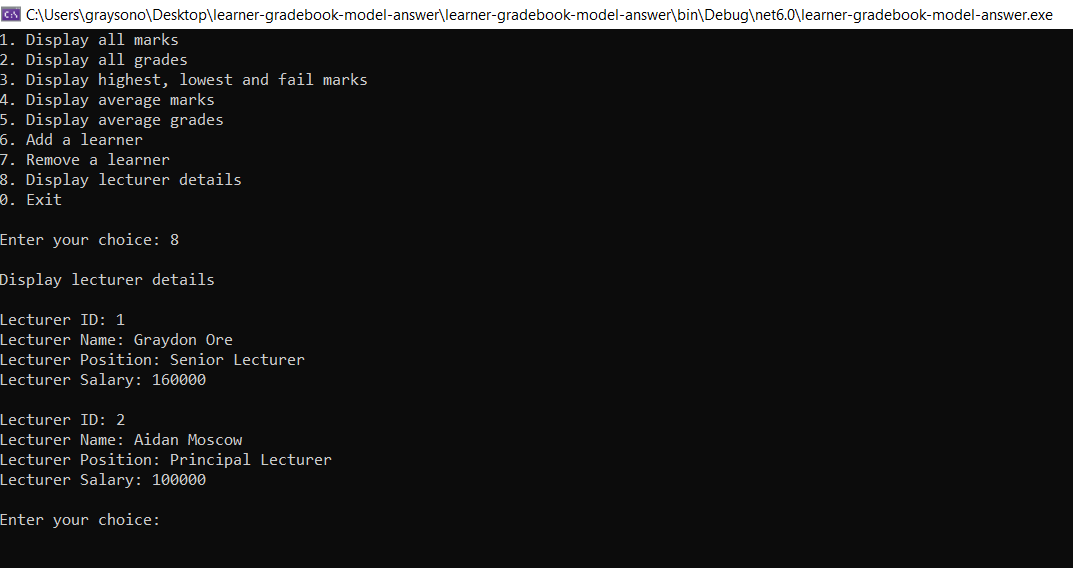
\includegraphics[width=150mm,height=75mm]{../../resources/img/project-1/9.PNG}
    \end{figure}
    \item When the user selects \textbf{0. Exit}, the app \textbf{must} exit. 
    \item 15 \textbf{unit tests} using \textbf{MSTest} which verify the functionality.
\end{itemize}

\newpage
\subsection*{Code Elegance - Learning Outcomes 1 \& 2  (45\%)}
\begin{itemize}
    \item Adhere to the principles of \textbf{OO}.
    \item Appropriate naming of classes, fields \& methods.
    \item Use of intermediate variables, constants \& try-catch blocks.
    \item Idiomatic use of control flow, data structures \& in-built functions.
    \item Efficient algorithmic approach.
    \item Sufficient modularity.
    \item Each class \textbf{must} have a header comment located immediately before its declaration.
    \item In-line comments where required. 
    \item App files, i.e., \textbf{.cs} files are formatted. 
    \item No dead or unused code.
\end{itemize}

\subsection*{Documentation \& Git Usage - Learning Outcomes 1 \& 2 (15\%)}
\begin{itemize}
    \item Provide the following in your repository \textbf{README.md} file:
    \begin{itemize}
        \item The app's class diagram created in \textbf{Visual Studio}. You must show all classes, fields, methods, properties \& relationships.
        \item How to run the \textbf{unit tests}.
        \item Known bugs if applicable.
    \end{itemize}
    \item Commit at least \textbf{20} times per week.
    \item Commit messages \textbf{must} be formatted using the convention discussed in \textbf{01-github-workflow-and-c\#-basics} \& reflect the context of each functional requirement change.
\end{itemize}

\end{document}